% !TeX spellcheck = nl_NL
\documentclass[a4paper,kul]{kulakarticle} %options: kul or kulak (default)

\usepackage[utf8]{inputenc}
\usepackage[dutch]{babel}

\date{Academiejaar 2021 -- 2022}
\address{
	Industriële Ingenieurswetenschappen \\
	BioTechnologie \\
	Inge Holsbeeks \& Hans Rediers}
\title{Samenvatting}
\author{Robbe Decapmaker}
\usepackage{hyperref}
\usepackage{graphicx}
\usepackage{amsmath, amssymb, amsthm}
\usepackage{siunitx}
\usepackage{flafter} 
\usepackage{pdfpages}



\begin{document}

\maketitle

\section*{Inleiding}

De samenvatting van BioTechnologie. \href{https://github.com/debber1/BioTech}{De source code is te vinden op Github.}\\
%DEZE ZIN IS ENKEL RELEVANT TIJDENS DE ONTWIKKELING VAN DIT DOCUMENT
\textbf{Dit document is een `work in progress', dit wil zeggen dat er (ongeveer) een wekelijkse update zal zijn. De meest recente versie zal altijd op Github staan!}
\tableofcontents
\newpage
\section{Koolhydraten}
Koolhydraten zijn essentieel voor biologisch leven. Grosso modo kunnen we 3 verschillende types onderscheiden: monosachariden, disachariden en polysachariden. Voor dat we deze types degelijk kunnen bespreken moet er eerst enkele afspraken vast gelegd worden rond naamgeving een voorstelling. We moeten ook nog enkele belangrijke opmerken maken rond de chemische fenomenen die zich voor doen bij koolhydraten. 
\subsection{Naamgeving}
Koolhydraten bestaan voornamelijk uit C, O en H atomen. Afhankelijk van de onderling gevormde bindingen kunnen we een onderscheid maken tussen twee soorten koolhydraten; de aldosen en ketonen. Het verschil tussen beiden wordt duidelijk gemaakt in figuur \ref{fig:aldehyde-keton}. Als een koolhydraat in bezit is van een aldehyde groep, noemen we hem een aldose. Als hij in bezit is van een keton groep, noemen we hem een ketose.
\begin{figure}[htbp]
	\centering
	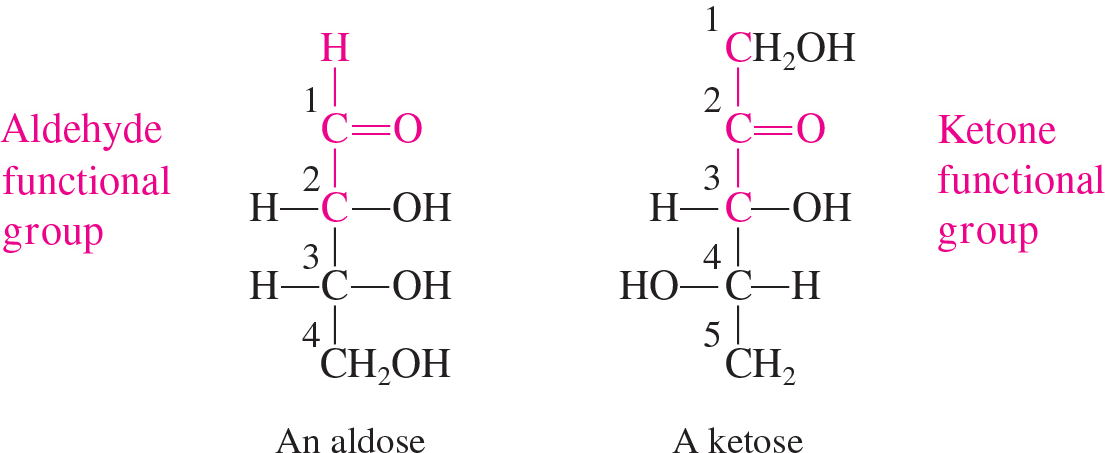
\includegraphics[width=0.7\linewidth]{Aldehyde-Keton}
	\caption[Aldehyden en ketonen]{Aldehyden en ketonen}
	\label{fig:aldehyde-keton}
\end{figure}\\
Naast de aanwezigheid van functionele groepen, maken we ook een onderscheid op basis van het aantal aanwezige koolstof atomen. De nummering en naamgeving van deze moleculen worden overgenomen uit de chemie zoals te zien is op figuur \ref{fig:examples-name}.
\begin{figure}[htbp]
	\centering
	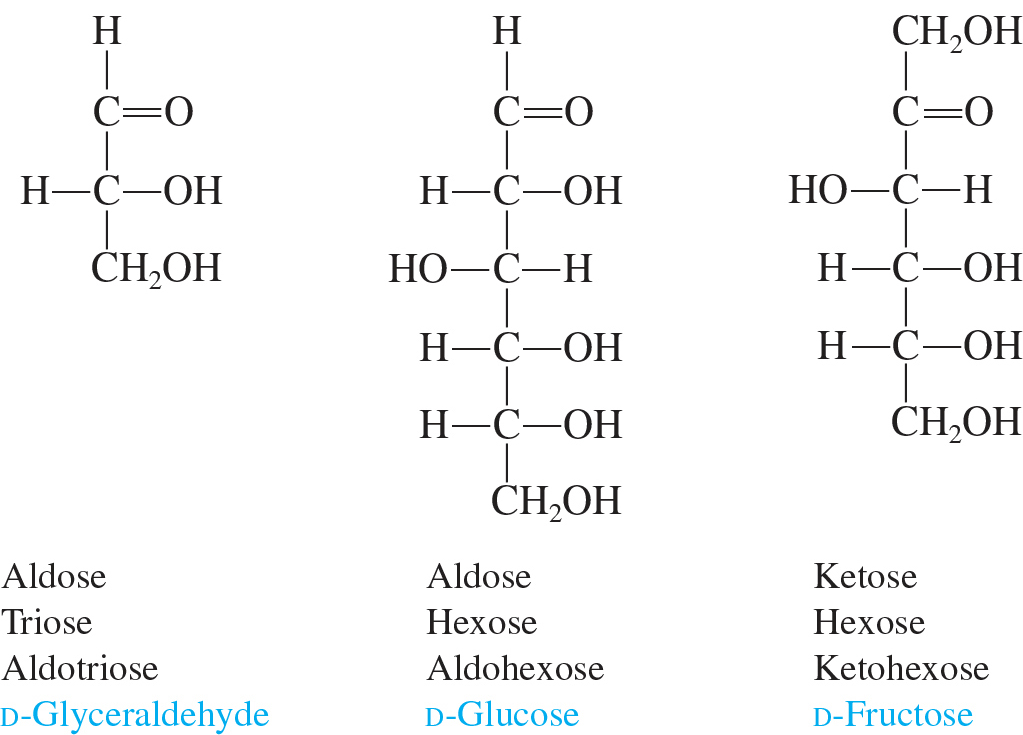
\includegraphics[width=0.6\linewidth]{examples-name}
	\caption[Naamgeving]{Voorbeelden van naamgeving}
	\label{fig:examples-name}
\end{figure}\\
Er zijn ook enkele koolhydraten die een triviale naam krijgen, zoals sacharose of fructose.

\subsection{Voorstellingen}
\subsection{Stereochemie}
\subsection{Reducerende koolhydraten}
\subsection{Monosachariden}
\subsubsection{Belangrijke monosachariden}
\subsubsection{Afgeleiden}
\subsection{Disachariden}
\subsubsection{Belangrijke disachariden}
\subsection{Polysachariden}
\subsubsection{Belangrijke polysachariden}
\section{Lipiden}
%Overzicht Schema slide 28
\subsection{Biologische functies van lipiden}
\subsection{Vetzuren}
\subsubsection{Structuur}
\subsubsection{(On)Verzadigde vetzuren}
\subsubsection{Cis- en Transvetzuren}
\subsubsection{Omega vetzuren}
\subsubsection{Reacties met vetzuren}
%Mooie samenvatting op slide 16
\subsection{Glyceriden}
\subsubsection{Structuur}
\subsubsection{Triglyceriden}
\subsubsection{Reacties}
\subsubsection{Fosfoglyceriden}
\subsection{Niet-glyceride lipiden}
\subsubsection{Sfingolipide}
\subsubsection{Steroïden}




\end{document}
